\documentclass{article}
\usepackage[polish]{babel}
\usepackage[T1]{fontenc}
\usepackage[utf8]{inputenc}
\usepackage{graphicx}
\usepackage{float}
\usepackage[bottom=0.5cm, right=1.5cm, left=1.5cm, top=1.5cm]{geometry}
\graphicspath{ {.} }

\title{%
  Cyberbezpieczeństwo - laboratoria 2 \\
  \large Kryptografia historyczna}
\author{Patryk Łuszczek 272707}
\date{\today}
\begin{document}
\maketitle
\newpage
\tableofcontents
\newpage

\section{Algorytmy historyczne - właściwości}
Tekst wykorzystany do analizy algorytmów:\\
Computer security, also known as cybersecurity or IT security, is the protection of computer systems from the theft or damage to their hardware, software or information, as well as from disruption or misdirection of the services they provide. The field is becoming more significant due to the increased reliance on computer systems, the Internet, wireless networks such as Bluetooth and Wi-Fi, and the growth of "smart" devices, including smartphones, televisions, and the various devices that constitute the "Internet of things". Owing to its complexity, both in terms of politics and technology, cybersecurity is also one of the major challenges in the contemporary world.

\subsection*{Zadanie 1.2 - właściwości poszczególnych algorytmów}
W celu przeprowadzenia badania zostały wykorzystane trzy algorytmy szyfrujące: Cezara, Vigenere, ADFGVX.\\\\

\textbf{Algorytm Cezara:}
Jest jednym z najprostszych algorytmów podstawieniowych. Polega na przesunięciu znaków tekstu jawnego o stałą wartość defniowaną przez klucz - literę alfabetu łacińskiego.
Klucz może przyjmować wartości od 0, w przypadku znaku A, do 25, w przypadku znaku Z. Z uwagi na małą przestrzeń możliwych kluczy, algorytm jest łatwy do złamania.\\\\
Dla przykładu zastosujemy algorytm Cezara dla wcześniej podanego tekstu, oraz klucza o wartości "L", co odpowiada przesunięciu tekstu jawnego o 11 znaków.
\begin{figure}[H]
    \centering
    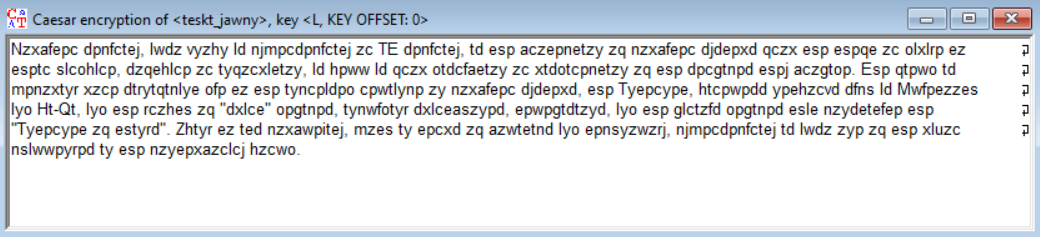
\includegraphics[width=\textwidth]{cezar_szyfr.png}
    \caption{Szyfrowanie algorytmem Cezara, ustawienia domyślne, klucz "L"}
\end{figure}
Jak można zauważyc, algorytm Cezara nie zmienia struktury tekstu, a jedynie przesuwa znaki o zadaną wartość.\\\\

\textbf{Algorytm Vigenere:}
Również jak algorytm Cezara, jest algorytmem podstawieniowym i nie zmienia struktury tekstu. Różni się jednak tym, że klucz nie jest pojedynczym znakiem, a ciągiem znaków. 
Kolejne znaki tekstu jawnego są przesuwane o wartość odpowiadające kolejnym znakom klucza. W przypadku, gdy klucz jest krótszy od tekstu jawnego, jest on powtarzany
do momentu zaszyfrowania całego tekstu. W przypadku używanego oprogramowania - CrypTool, klucz może mieć maksymalnie 1024 znaków. W przypadku klucza o takiej długości
istnieje 26\^1024 możliwych kombinacji, co czyni algorytm Vigenere dużo bardziej skomplikowanym od algorytmu Cezara.

\begin{figure}[H]
    \centering
    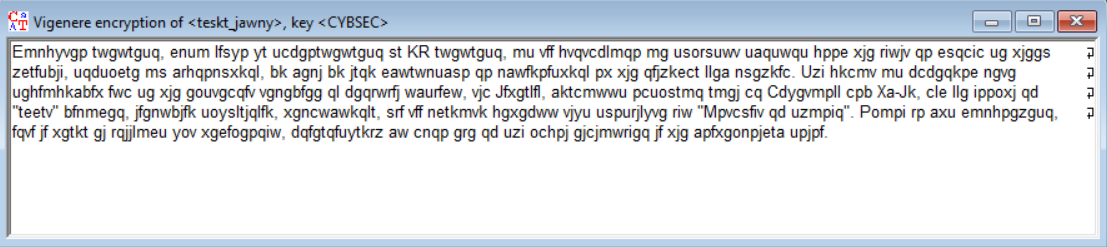
\includegraphics[width=\textwidth]{vigenere_szyfr.png}
    \caption{Szyfrowanie algorytmem Vigenere, ustawienia domyślne, klucz "CYBSEC"}
\end{figure}

\textbf{Algorytm ADFGVX:}
Algorytm ADFGVX jest algorytmem podstawieniowym i transpozycyjnym. Polega na przekształceniu każdej litery tekstu jawnego na parę znaków ze zbioru ADFGVX za pomocą zmodyfikowanej tablicy 
Polibiusza. Następnym krokiem jest wybranie klucza, za pomocą którego zostanie przeprowadzona transpozycja szyfogramu. Macierz wykorzystana do szyfrowania jest wypełniona kolejnymi literami alfabetu łacińskiego oraz
cyframi od 0 do 9. W związku z tym, tablica wykorzystywana do szyfrowania może zostać wypełniona na 36! różnych kombinacji. Klucz powinien składać się natomiast z maksymalnie 26 unikalnych znaków.
\begin{figure}[H]
    \centering
    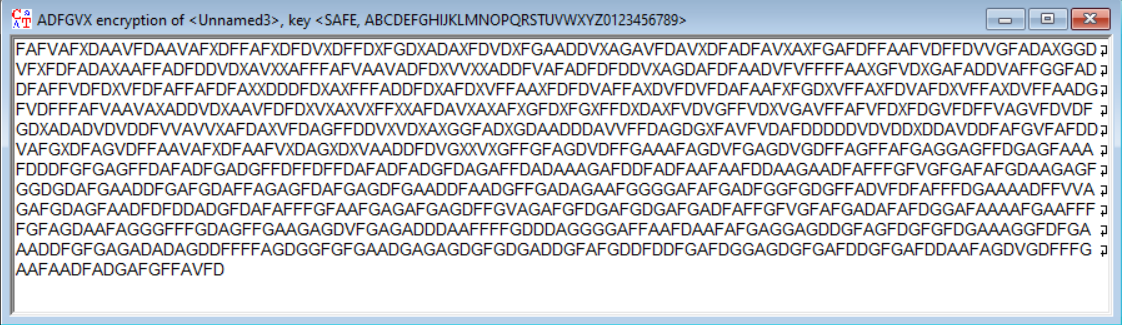
\includegraphics[width=\textwidth]{adfgvx_szyfr.png}
    \caption{Szyfrowanie algorytmem ADFGVX, ustawienia domyślne, klucz "SAFE"}
\end{figure}
Jak można zauważyć struktura tekstu została zmieniona, zostały pominięte znaki interpunkcyjne oraz spacje - ma to związek z zwiększeniem bezpieczeństwa algorytmu.
W porównaniu do wczeńsniej omawianych algorytmów, ADFGVX wygląda na bardziej skomplikowany i bezpieczny algorytm szyfrujący.

\subsection*{Pytanie 1.3 - szyfrowanie wielokrotne}
\textbf{Treść:}
Co możemy powiedzieć o szyfrowaniu wielokrotnym w kontekście algorytmów historycznych? Jak takie działanie wpływa na możliwość
rozszyfrowania tekstu. Odpowiedź na to pytanie zilustruj wynikiem eksperymentu przeprowadzonego w Cryptool.\\\\
Szyfrowanie wielokrotne algorytmami przedstawionymi powyżej.

\begin{figure}[H]
    \centering
    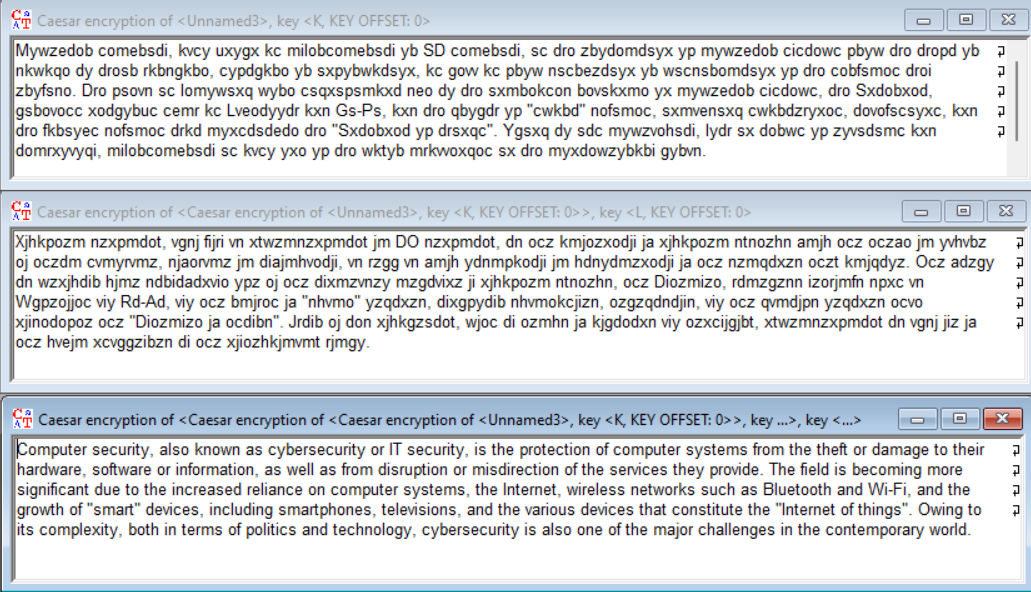
\includegraphics[width=\textwidth]{cezar_wielokrotne.png}
    \caption{Szyfrowanie algorytmem Cezara, ustawienia domyślne, klucze "K","L","F"}
\end{figure}

\begin{figure}[H]
    \centering
    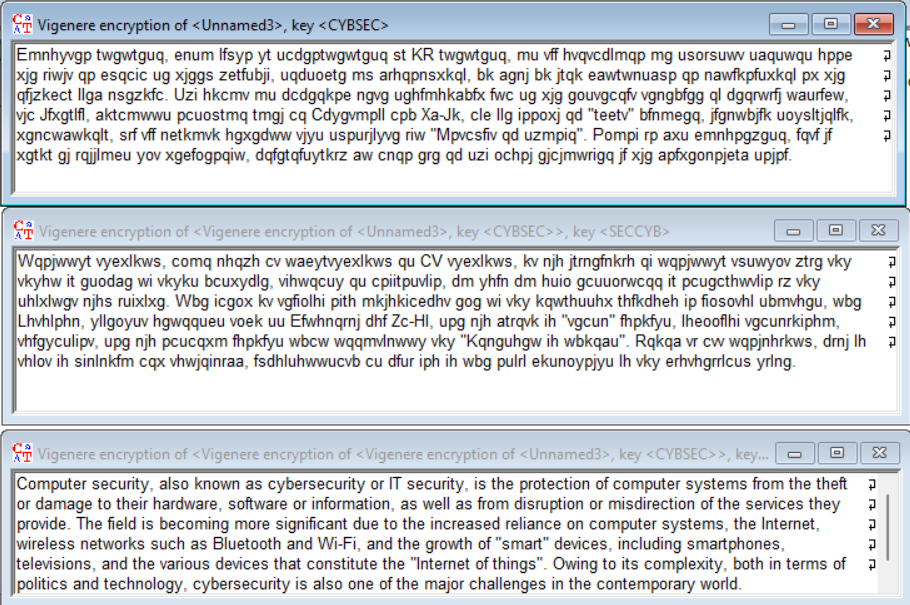
\includegraphics[width=\textwidth]{vinegre_wielokrotne.png}
    \caption{Szyfrowanie algorytmem Vigenere, ustawienia domyślne, klucz "CYBSEC","SECCYB","GYXGYX}
\end{figure}

\begin{figure}[H]
    \centering
    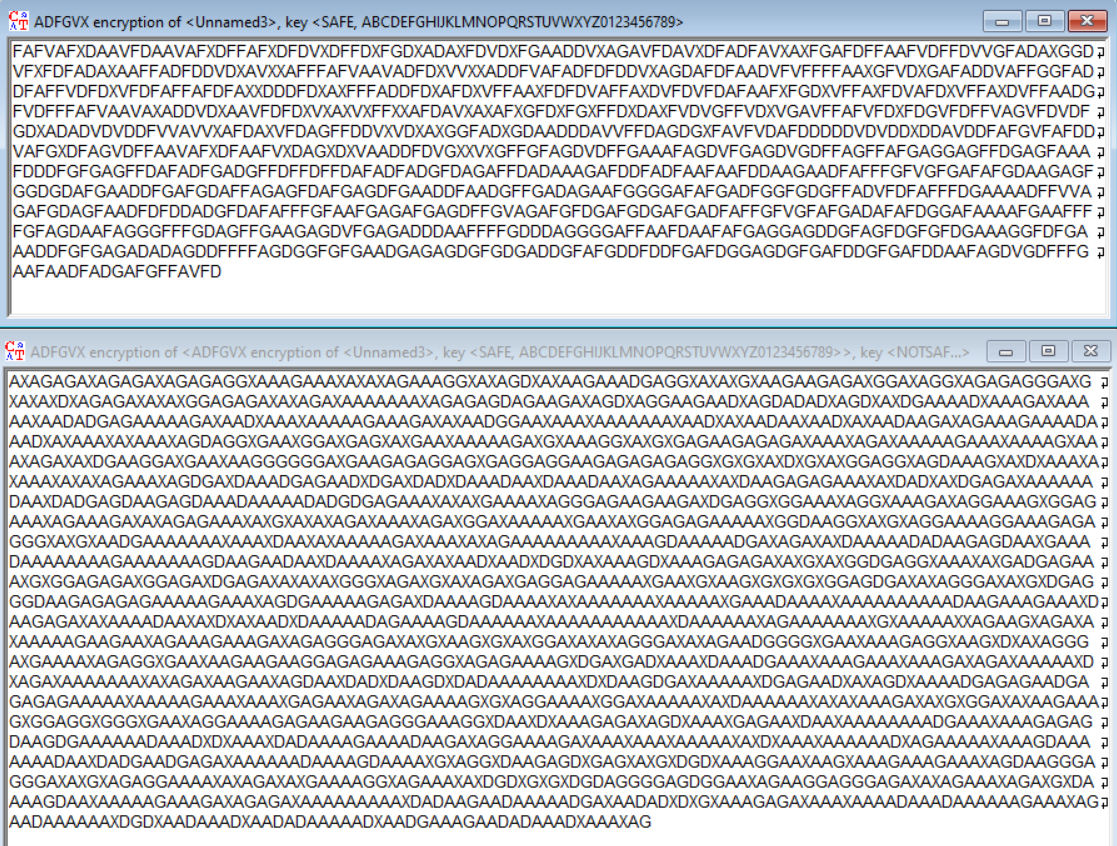
\includegraphics[width=\textwidth]{adfgvx_wielokrotne.png}
    \caption{Szyfrowanie algorytmem ADFGVX, ustawienia domyślne, klucz "SAFE","NOTSAFE"}
\end{figure}

\textbf{Wnioski:}
\begin{itemize}
    \item Szyfr Cezara \\
    Szyfrowanie wielokrotne algorytmem Cezara nie zwiększa bezpieczeństwa tekstu. Ma to związek z prostotą działania sposobu szyfrowania. Dla wcześniej pokazanego przykładu zostało zastosowane
    przeunięcie o 10 znaków, następnie o 11 znaków a finalnie o 5 znaków. Jest to równoznaczne z przesunięciem o 26 znaków, co oznacza powrót do tekstu jawnego.
    \item Szyfr Vigenere \\
    W przypadku tego algorytmu, szyfrowanie wielokrotne może nieco zwiększyć bezpieczeństwo tekstu. Zwłaszcza jeśli klucze będą długie i unikalne. Jednak w przypadku
    zastosowania krótkich lub powtarzających się kluczy, algorytm szybko staje się łatwy do złamania.
    \item Szyfr ADFGVX \\
    Algorytm ADFGVX jest najbardziej skomplikowany z omawianych algorytmów. Szyfrowanie wielokrotne zwiększa bezpieczeństwo tekstu w większym stopniu niż
    w przypadku algorymtu Cezara i Vigenere. Ma to związek z dużą ilości możliwych kombinacji podstawień oraz dodatkowego kroku transpozycji szyfrogramu.
    W związku z tym algorytm ADFGVX jest najbezpieczniejszym z omawianych algorytmów. 
\end{itemize}

\subsection*{Pytanie 1.4 - bezpieczeństwo algorytmów}
\textbf{Treść:}
Który z przetestowanych algorytmów może być uznany za silniejszy i dlaczego?\\\\
W przypadku omawianych algorytmów zdecydowanie najbezpieczniejszy jest algorytm ADFGVX.
Ma to związek z większą złożonością algorytmu. Przedewszystkim poszczególne znaki nie są przesuwane o stałą wartość, a zamieniane na parę znaków.
Następnie szyfrogram jest transponowany za pomocą klucza, co dodatkowo utrudnia próby złamania szyfru. W związku z tym analiza szyfrogramu jest znacznie trudniejsza.


\section{Analiza własności dostępnych algorytmów}

\subsection*{Zadanie 2.1 - entropia tekstu jawnego dla różnych języków}
\begin{table}[H]
    \centering
    \begin{tabular}{|c|c|}
        \cline{1-2}
        \textbf{Język} & \textbf{Entropia}  \\ \cline{1-2}
        Angielski      & 4.10               \\ \cline{1-2}
        Polski         & 4.25               \\ \cline{1-2}
        Czeski         & 4.29               \\ \cline{1-2}
        Francuski      & 4.01               \\ \cline{1-2}
    \end{tabular}
    \caption{Porównanie entropii dla języków: angielski, polski, czeski, francuski}
\end{table}
\subsection*{Zadanie 2.2 - entropia dla różnych algorytmów}
\begin{table}[H]
    \centering
    \begin{tabular}{|c|c|}
    \hline
    \textbf{Algorytm}     & \textbf{Entropia} \\ \hline
    \textbf{jawny}        & 4.10              \\ \hline
    \textbf{Cezar}        & 4.10              \\ \hline
    \textbf{ADFGVX}       & 2.42              \\ \hline
    \textbf{homofonów}    & 7.58              \\ \hline
    \textbf{permutacji}   & 4.10              \\ \hline
    \textbf{Vigenere(13)} & 4.60              \\ \hline
    \textbf{Vigenre(4)}   & 4.49              \\ \hline
    \textbf{Hill(2x2)}    & 4.61              \\ \hline
    \textbf{Hill(5x5)}    & 4.68              \\ \hline
    \end{tabular}
    \caption{Porównanie entropii dla algorytmów: Cezara, ADFGVX, homofonów, permutacji, Vigenere, Hilla}
\end{table}
\subsection*{Zadanie 2.3 - histogramy tekstu jawnego dla różnych języków}
\begin{figure}[H]
    \centering
    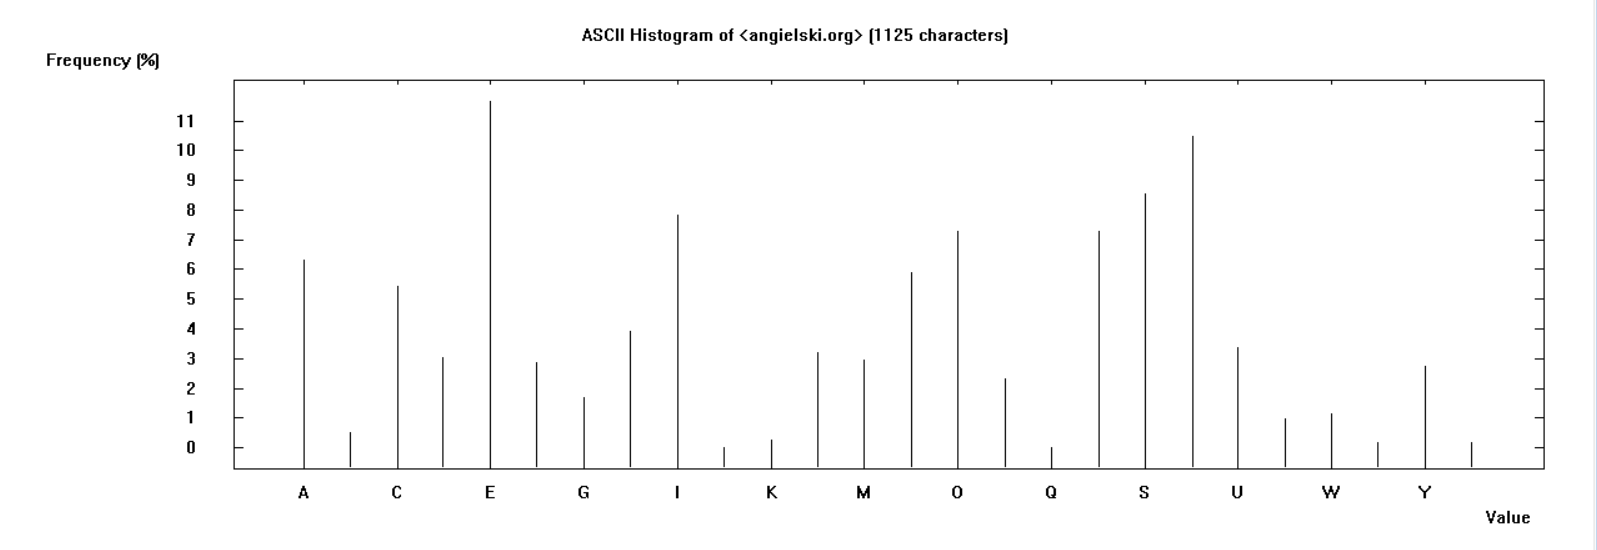
\includegraphics[width=\textwidth]{angielski_histogram.png}
    \caption{Histogram dla tekstu jawnego w języku angielskim}
\end{figure}
\begin{figure}[H]
    \centering
    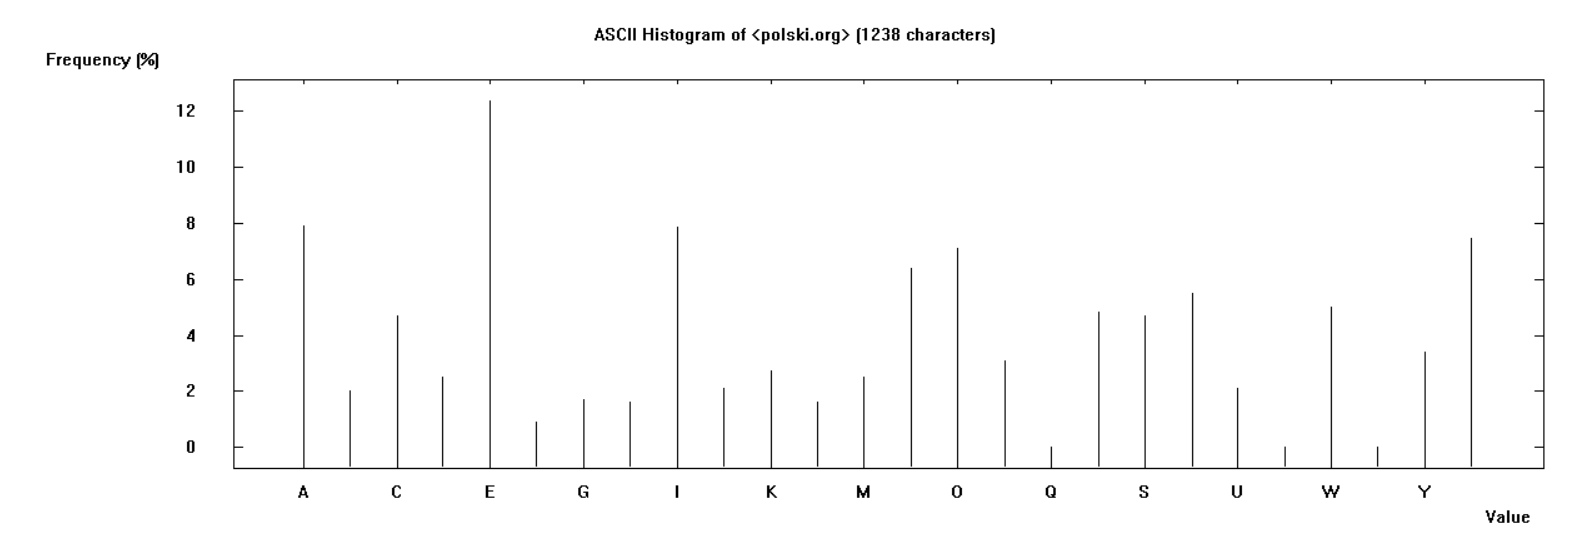
\includegraphics[width=\textwidth]{polski_hisogram.png}
    \caption{Histogram dla tekstu jawnego w języku polskim}
\end{figure}
\begin{figure}[H]
    \centering
    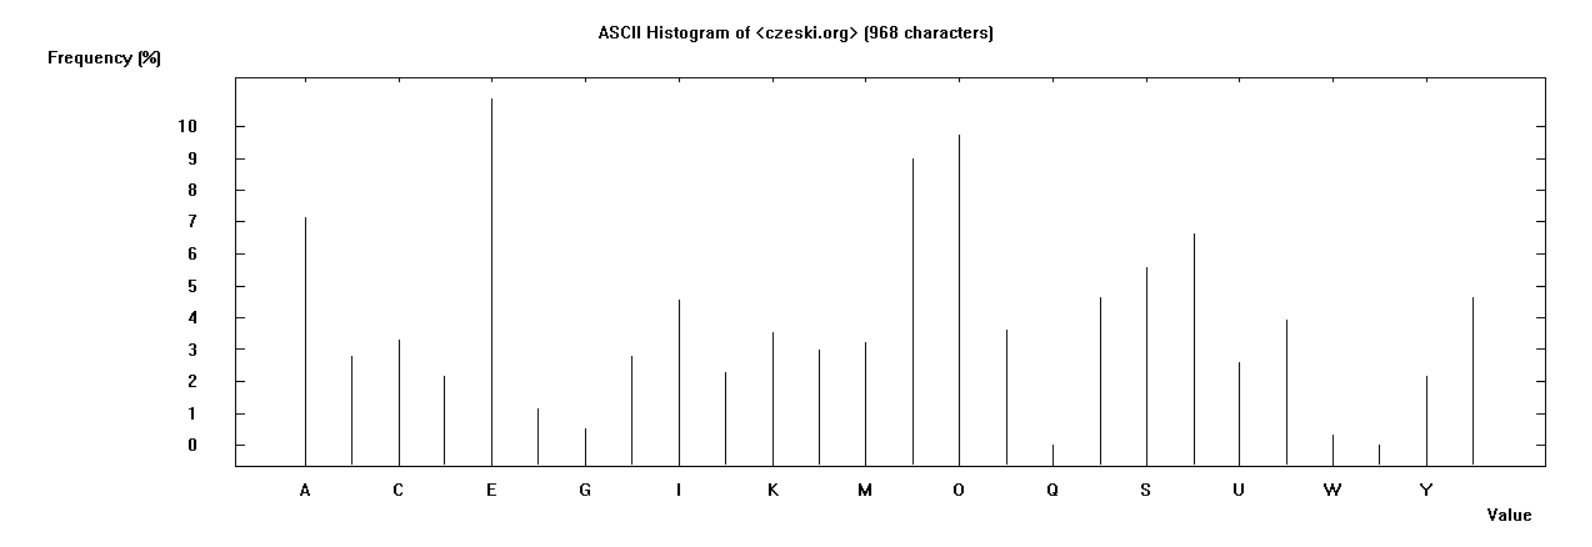
\includegraphics[width=\textwidth]{czeski_hisogram.png}
    \caption{Histogram dla tekstu jawnego w języku czeskim}
\end{figure}
\subsection*{Zadanie 2.4 - porównanie histogramu tekstu jawnego i zaszyfrowanego}
\begin{figure}[H]
    \centering
    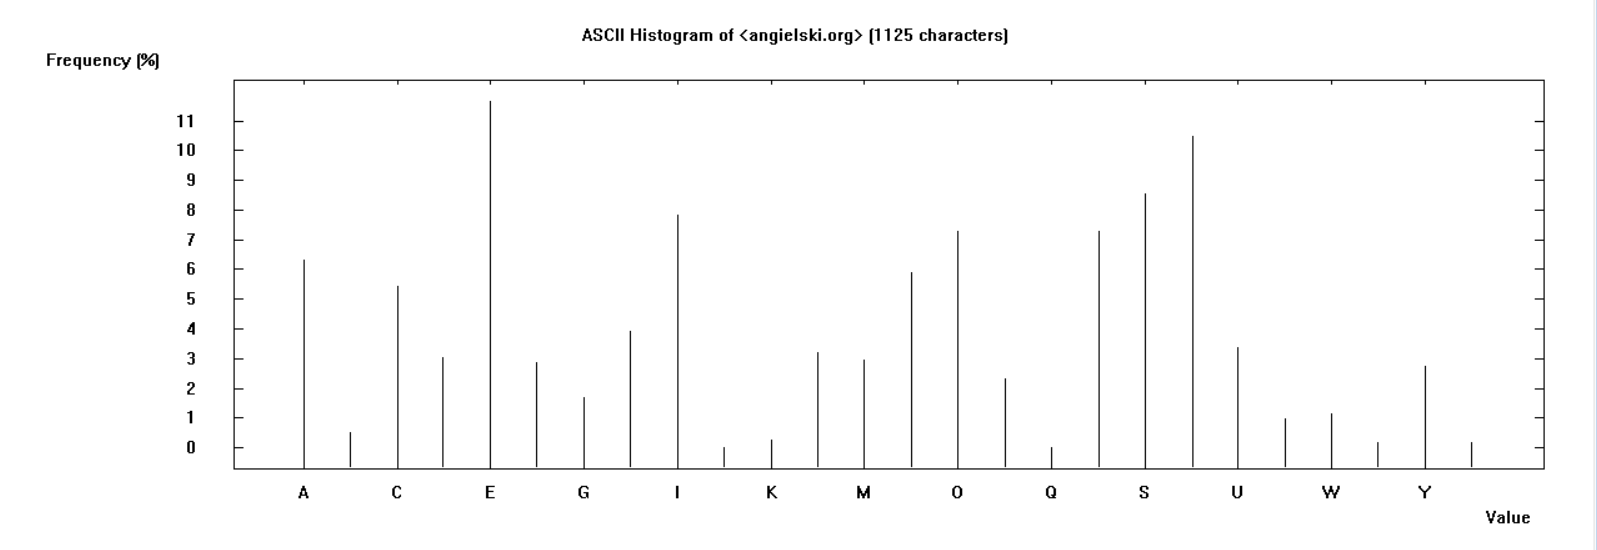
\includegraphics[width=\textwidth]{angielski_histogram.png}
    \caption{Histogram dla tekstu jawnego w języku angielskim}
\end{figure}

\begin{figure}[H]
    \centering
    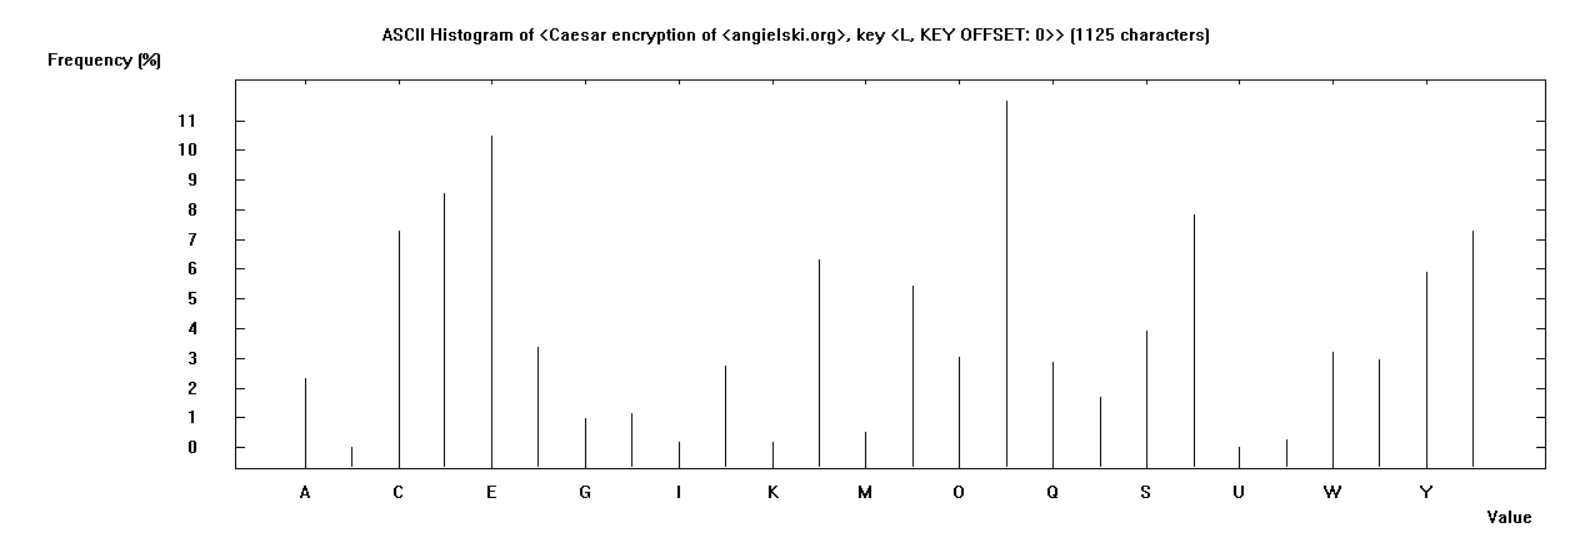
\includegraphics[width=\textwidth]{cezar_hisogram.png}
    \caption{Histogram dla tekstu zaszyfrowanego algorytmem Cezara}
\end{figure}

\begin{figure}[H]
    \centering
    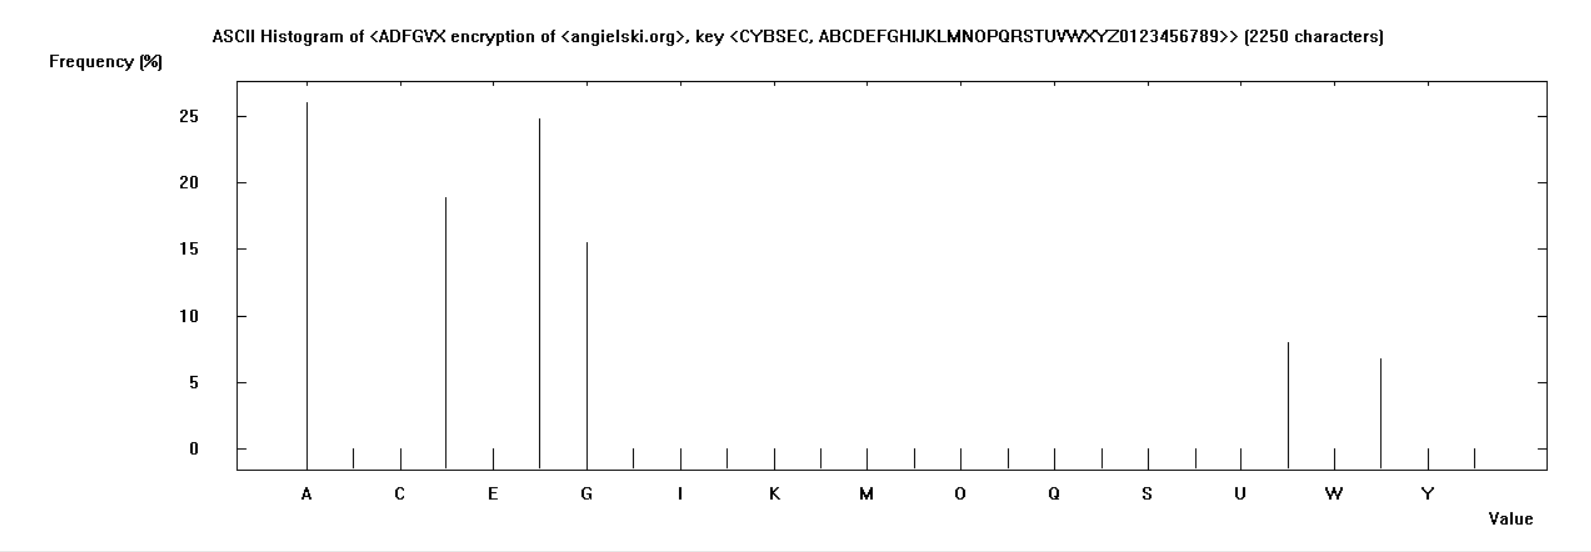
\includegraphics[width=\textwidth]{adfgvx_hisogram.png}
    \caption{Histogram dla tekstu zaszyfrowanego algorytmem ADFGVX}
\end{figure}

\begin{figure}[H]
    \centering
    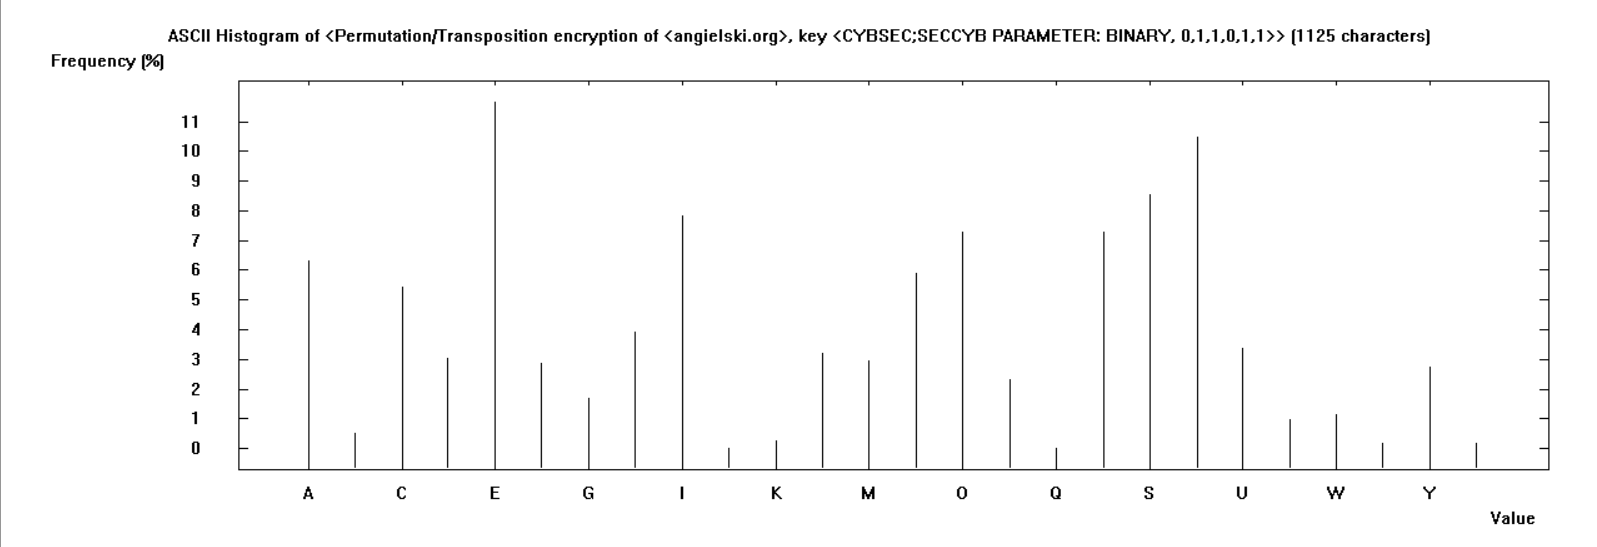
\includegraphics[width=\textwidth]{permutacyjny_histogram.png}
    \caption{Histogram dla tekstu zaszyfrowanego algorytmem permutacyjnym}
\end{figure}
\subsection*{Czym jest ngram?}
Ngram to ciąg znaków o określonej długości - n. Dzięki analizie tekstu za pomocą ngramów można określić częstotliwość występowania poszczególnych znaków, w 
przypadku histogramu, lub ciągu n znaków. Pozwala to na znalezienie najczęściej występujących znaków lub ciągów znaków w szyfrogramie.

\subsection*{Pytanie 2.8 - zmiana parametrów}
\textbf{Treść: } Jak zmieniają się obserwowane parametry w zadaniach od 1 do 7?\\\\
W przypadku szyfrowania algorytmem Cezara oraz permutacji możemy zauważyć, że entropia tekstu zaszyfrowanego jest taka sama jak dla tekstu jawnego - 4.10.
Oznacza to, że algorytmy te nie wprowadzają znaczącej losowości podczas szyfrowania. Algorytm ADFGVX cechuje się najniższą entropią spośód wszystkich algorytmów - 2.42.
Ma to związek z ograniczoną liczbą znaków w szyfrogramie. Niska entropia może oznaczać, że szyfrogram jest bardziej przewidywalny i podatny na próby złamania szyfru.
W przypadku algorymtu homofonów możemy zaobserwować największą entropię wynoszącą 7.58. Ma to związek z większą ilością znaków w szyfrogramie, co sprawia że szyfrogram jest bardziej skomplikowany
i trudniejszy do złamania. Algorytm Vigenera o długości klucza równej 4 cechuje się mniejszą entropią niż w przypadku klucza o długości 13. Oznacza to, że dłuższy klucz zapewnia nieco większe bezpieczeństwo.
Natomiast algorytm Hilla o wymiarze macierzy 2x2 wykazał entropię równą 4.61, a zwiększenie macierzy do rozmiaru 5x5 spowodowało dodatkowe zwiększenie entropii szyfrogramu.\\\\

Histogram tekstu jawnego wskazywał, że najczęsciej występującym znakiem jest litera "E". Po zaszyfrowaniu tekstu algorytmem Cezara najczęściej występującym
znakiem jest "P" co oznacza, że tekst został przesunięty o 11 znaków. W przypadku algorytmu ADFGVX najczęściej występującym znakiem stała się litera "A". Ma
to związek z ograniczoną liczbą znaków w szyfrogramie, które ograniczają się do liter ze zbioru "ADFGVX". Histogram dla tekstu zaszyfrowanego algorytmem permutacyjnym
nie różni się od hisogramu tekstu jawnego. Oznacza to, że algorytm jedynie przestawia znaki w tekście.

\subsection*{Pytanie 2.9 - wykorzystanie narzędzi w celu określenia algorytmu}
\textbf{Treść: } W jaki sposób można wykorzystać narzędzia analizy tekstu dostępne w CrypTool do określenia
algorytmu szyfrowania dla danego zaszyfrowanego tekstu?\\\\
W celu określenia algorytmu szyfrowania można skorzystać z entropii. W przypadku algorytmów, które wprowadzają większą losowość do tekstu zaszyfrowanego, entropia
będzie wyższa. Jeśli jednak entropia będzie niska, może to wskazywać na wykorzystanie algorytmu ADFGVX lub innego algorytmu, który wprowadza ograniczoną liczbę znaków do szyfrogramu.
Kolejnym sposobem jest analiza struktury tekstu. Jeśli tekst zaszyfrowany zachowuje regularną strukturę, może to wskazywać na zastosowanie prostego algorytmu podstawieniowego, takiego jak
algorytm Cezara czy Vigenere. Zastosowanie ngramów pozwala na analize częstotliwości występowania poszczególnych znaków lub ciągów znaków. Jeśli pewne ngramy występują często,
może to wskazywać na wykorzystanie algorytmu, który nie wprowadza dużej losowości w tekście. Jeśli natomiast ngramy występują bardzo rzadko, może to wskazywać na zastosowanie
bardziej złożonego algorytmu, w szczególności takiego, w którym jeden znak może zostać zaszyfrowany na kilka sposobów np. algorytm homofonów.

\subsection*{Pytanie 2.10 - wykorzystanie narzędzi w celu określenia klucza}
\textbf{Treść: } W jaki sposób można wykorzystać narzędzia analizy tekstu dostępne w programie CrypTool
do ustalenia hasła używanego szyfrowania?\\\\
W celu ustalenia klucza można skorzystać z analizy częstotliwości występowania poszczególnych znaków w tekście zaszyfrowanym. Sprawdzi się to przede wszystkim
w przypadku zastosowania algorytmu Cezara. Najczęściej występujący znak w tekście zaszyfrowanym może odpowiadać znakowi najczęściej występującym w danym języku.
Analiza ngramów również może pomóc w ustaleniu klucza, jeśli porówna się ją z ngramami często występującymi w danym języku.
\section{Analiza plików}
\subsection*{Zadanie 3.1 - analiza wykorzystanego szyfru}
\subsubsection*{Plik 1\_1.txt}
\begin{figure}[H]
    \centering
    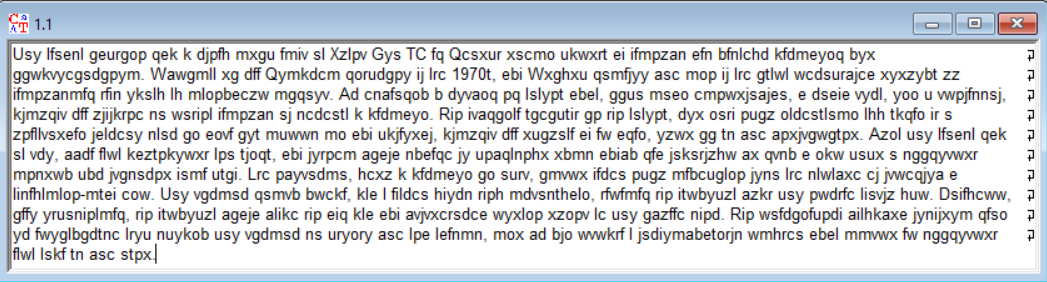
\includegraphics[width=\textwidth]{1_1.png}
    \caption{Szyfrogram plik 1\_1.txt}
\end{figure}
\textbf{Analiza:}
\begin{itemize}
    \item Struktura tekstu jest regularna, przypomina tekst zaszyfrowany prostym algorytmem podstawieniowym: Cezara lub Vigenere
    \item Analiza hisogramu wykazała, że najczęściej występującym znakiem jest litera "S". Jeśli przyjmiemy, że tekst został napisany w języku angielskim, może to wskazywać
    na to, że zaszyfrowana litera "S" odpowiada literze "E" w tekście jawnym, ponieważ jest to najczęściej występująca litera w języku angielskim.
    \item Analiza trigramu wskazuje, że najczęściej występującym trigramem jest ciąg "RIP" (8) oraz "USY" (6). Mogą to być odpowiedniki angielskich wyrazów "AND" oraz "THE".
    \item W tekście występują pojedyncze znaki przed dłuższymi "wyrazami". Wygląda to tak jakby był odpowiednikami "a" przed angielskim rzeczownikiem. Również występują
    digramy mogące być odpowiednikami "an", "in", "on", "is" lub "to". Jednak odpowiednie znaki w tych digramach nie odpowiadają sobie w zaszyfrowanym tekście, więc można
    wynioskować, że tekst został zaszyfrowany kluczem, który nie jest stały - nie ma jednolitego przesunięcia znaków.
    \item W związku z powyższym można wywnioskować, że tekst został najprawdopobniej zaszyfrowany algorytmem \textbf{Vigenere}.
\end{itemize}

\subsubsection*{Plik 1\_2.txt}
\begin{figure}[H]
    \centering
    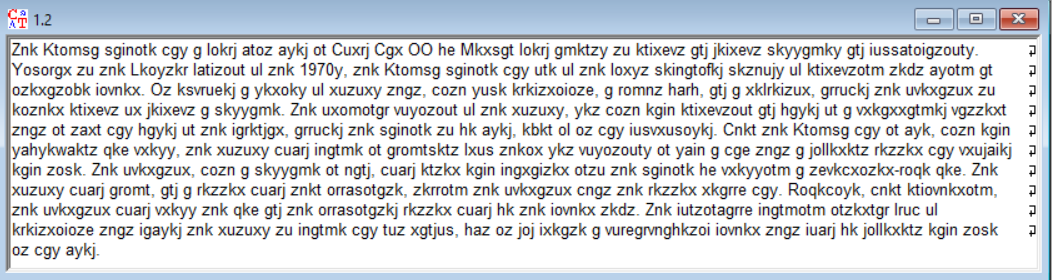
\includegraphics[width=\textwidth]{1_2.png}
    \caption{Szyfrogram plik 1\_2.txt}
\end{figure}
\textbf{Analiza:}
\begin{itemize}
    \item Struktura tekstu jest regularna, w zasadzie taka sama jak w przypadku poprzedniego pliku. Oznacza to, że został wykorzystany prosty algorytm podstawieniowy, który
    nie zmienia struktury tekstu.
    \item Analiza histogramu wykazałą, że najczęściej występującym znakiem jest znak, "K". Jeśli przyjmiemy, że tekst został napsiany w języku angielskim, powinno to odpowiadać lierze "E"
    tekstu jawnego.
    \item Analiza ngramów, w szczególności trigramów wykazała znaczącą dominację trigramu "ZNK" (26) ponad innymi trigramami. Oznacza to, że najprawdopobniej został zastosowany
    algorytm, który szyfruje znaki w sposób stały. 
    \item W związku z powyższymi argumentami można przyjąć, że został wykorzystany algorytm \textbf{Cezara}.
\end{itemize}
\subsubsection*{Plik 1\_3.txt}
\begin{figure}[H]
    \centering
    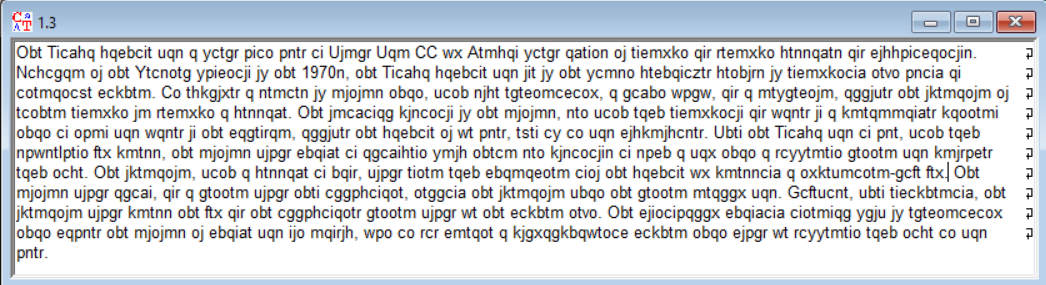
\includegraphics[width=\textwidth]{1_3.png}
    \caption{Szyfrogram plik 1\_3.txt}
\end{figure}
\textbf{Analiza:}
\begin{itemize}
    \item Struktura tekstu jest równie regularna jak w przypadku poprzednich plików. 
    \item Występują trigramy w takiej samej liczności jak w przypadku poprzedniego pliku, jednak są one inne.
    \item Można przyjąć, że został wykorzystany algorytm Vigenere o długim kluczu, lub algorytm Substitution.
\end{itemize}

\subsection*{Zadanie 3.2 - próba złamania szyfru}
\subsubsection*{Plik 2\_1.txt}
\begin{figure}[H]
    \centering
    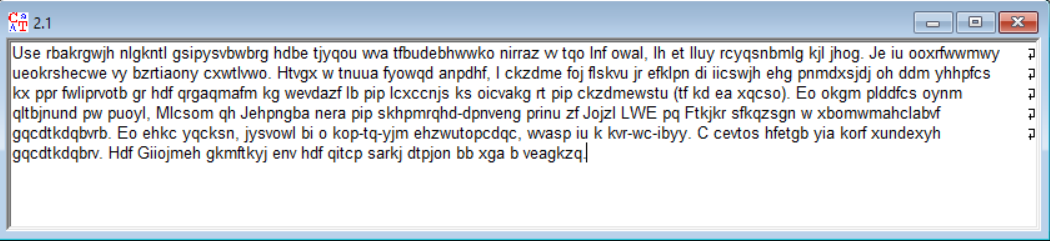
\includegraphics[width=\textwidth]{2_1.png}
    \caption{Szyfrogram plik 2\_1.txt}
\end{figure}
\textbf{Analiza: }
\begin{itemize}
    \item Reularna struktura pliku, przypomina tekst zaszyfrowany prostym algorytmem podstawieniowym typu Cezara lub Vigenere ewentualnie algorytmem Hilla.
    \item Brak dominującego trigramu - klucz najprawdopobnie nie jest stały (przyjmując, że jest to język angielski) więc wyklucza to wykorzystanie algorytmu
    Cezara. Wykryte zostało wiele ngramów o jednakowej częstotliwości występowania, wskazuje to na możliwe wykorzystanie algorytmu Vigenere.
    \item Test autokorelacji wykazuje, że najprawdopobniej został użyty klucz o długości 11 znaków - wykres wskazuje na zwiększoną liczbę
    nakładających się znaków w przypadku przesunięcia o wieloktorności liczby 11.
\end{itemize}

\begin{figure}[H]
    \centering
    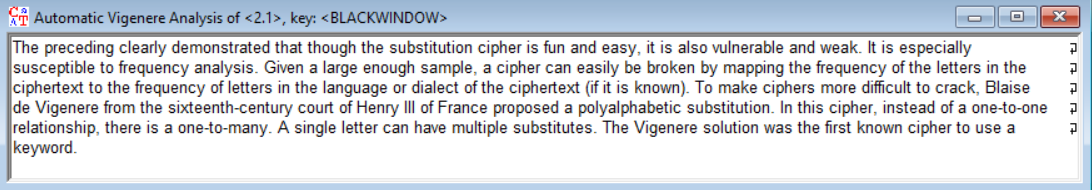
\includegraphics[width=\textwidth]{2_1_rozszyfrowany.png}
    \caption{Rozszyfrowany tekst pliku 2\_1.txt}
\end{figure}

\textbf{Eksperyment: }
\begin{itemize}
    \item Przyjmijmy, że klucz ma długość 11 znaków, a pierwszy wyraz szyfrogramu to "the". Użyjemy więc klucza "BLAAAAAAAAA" w celu próby odszyfrowania początku tekstu
    i pozostawienia reszty szyfrogramu bez zmian.
    \item Dalsza próba odgadnięcią klucza ręcznie może być bardzo czasochłonna. Zostało więc wykorzystane narzędzie dostępny w CrypTool do automatycznego złamania szyfru.
    W wyniku tego zabiegu odnaleziono klucz \textbf{BLACKWINDOW}, zatem poprawnie odgatnięto trzy pierwsze znaki klucza.
\end{itemize}

\subsubsection*{Plik 2\_2.txt}
\begin{figure}[H]
    \centering
    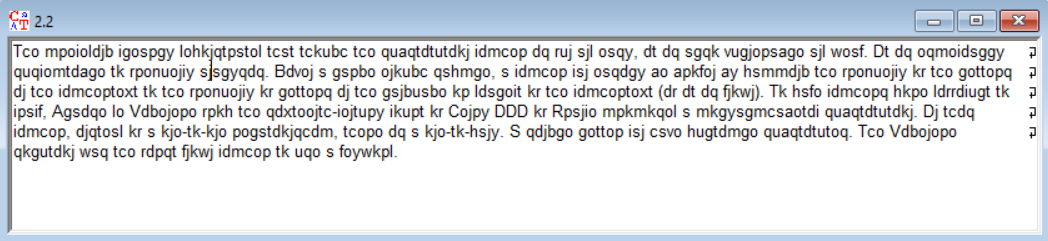
\includegraphics[width=\textwidth]{2_2.png}
    \caption{Szyfrogram plik 2\_2.txt}
\end{figure}

\textbf{Analiza: }
\begin{itemize}
    \item W przypadku tego szyfrogramu również występuje regularna struktura, przypomina tekst z poprzedniego pliku
    \item Analiza korelacji wykazuje brak cykliczności, jest to najprawdopobniej algorytm Hilla lub Substitution.
\end{itemize}

\textbf{Eksperyment: }
\begin{itemize}
    \item Narzędzie automatycznego rozwiązywania szyfru nie było w stanie odgadnąć klucza dla algorytmu Hilla, w przypadku algorytmu Substitution tekst został
    częściowo rozszyfrowany.
\end{itemize}
\begin{figure}[H]
    \centering
    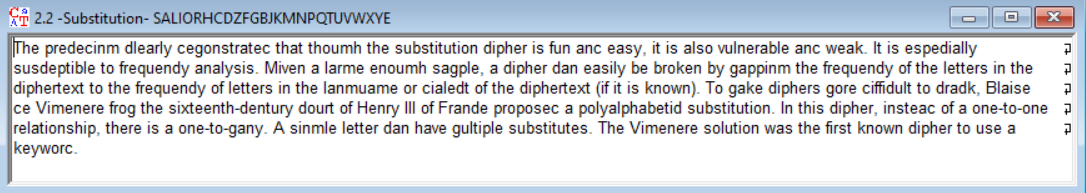
\includegraphics[width=\textwidth]{2_2_rozszyfrowany.png}
    \caption{Częściowo rozszyfrowany tekst pliku 2\_2.txt}
\end{figure}
\subsubsection*{Plik 2\_3.txt}
\begin{figure}[H]
    \centering
    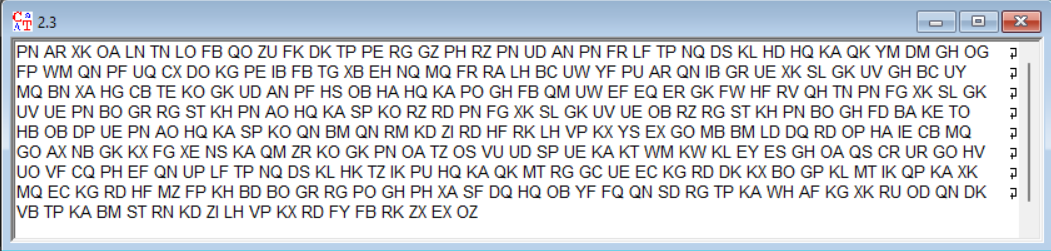
\includegraphics[width=\textwidth]{2_3.png}
    \caption{Szyfrogram plik 2\_3.txt}
\end{figure}
\textbf{Analiza: }
\begin{itemize}
    \item Struktura tekstu przypomina użycie algorytmu Playfair
\end{itemize}
\textbf{Eksperyment: }
\begin{itemize}
    \item Próba złamania szyfru za pomocą narzędzi dostępnych w CrypTool zakończyła się niepowodzeniem
\end{itemize}

\subsection*{Pytanie 3.4 - siła algorytmu}
\textbf{Treść:} Od czego zależy siła algorytmu? \\\\
Siła algorytmu szyfrującego zależy przede wszystim od:
\begin{itemize}
    \item \textbf{Złożoności i przetrzeń klucz} - im dłuższy i mniej przewidywalny klucz tym zazwyczaj algorytm jest bezpieczniejszy. Krótkie i proste klucze są podatne na
    ataki brute force.
    \item \textbf{Złożoności działania algorytmu} - proste algorytmy podstawieniowe, takie jak szyfr Cezara lub algorytm Vigenre są łatwiejsze do złamania
    w porównaniu do bardziej skomplikowanych algorytmów, takich jak np. algorytm ADFGVX, który oprócz podstawienia stosuje transpozycje lub algorytm homofonów,
    który wpowadza dużą losowość szyfrogramu
    \item \textbf{Losowości} algorytmy, które wprowadzają większą losowość i nieregularność do szyfrogramu są bezpieczniejsze
\end{itemize}
\subsection*{Pytanie 3.5 - zwiększenie bezpieczeństwa algorytmów}
\textbf{Treść: } W jaki sposób można zwiększyć siłe szyfrowania znanych szyfrów?\\\\
W celu zwiększenia siły szyfrowania, powinno się stosować długie skomplikowane klucze, które będą w miare możliwości unikalne i niepowtarzalne. W przypadku
niektórych algorytmów wielokrotne szyfrowanie różnymi kluczami może znacząco podnieść bezpieczeństwo szyfru. Jeśli algorytm wykorzystuje macierze do szyfrowania, stosowanie większych macierzy wypełnionych w bardziej nieprzewidywalny
sposób jest wskazane. 
\end{document}